
\chapter{Rule Learning System Details} \label{chap:algo}

This chapter will introduce the proposed classification rule learning system and provide implementation details that are aligned to the goals stated in Chapter \ref{chap:intro}.
Section \ref{chap:algo:overview} gives a high-level overview of the proposed system and provides context on the broad choices made.
Section \ref{chap:algo:binning} describes the feature generation procedure used in this work.
Section \ref{chap:algo:whypriori} describes the rule learning algorithm that was chosen and why.
Section \ref{chap:algo:weightcov} describes the Weighted Covering Algorithm and why it was chosen for this system.
Section \ref{chap:algo:proposed} covers the overall system and how it is evaluated.

\section{Overview} \label{chap:algo:overview}
The proposed system is called \Name (\Abb) and has two stages of interest, one is a classification rule learning system (seen in Figure \ref{fig:covering}), and the other is a higher level covering loop that operates on rule sets (Figure \ref{fig:highlevel}). Both stages are designed to be as simple as possible to enable a transparent view into their operation. 



\begin{figure}[h]
    \centering
    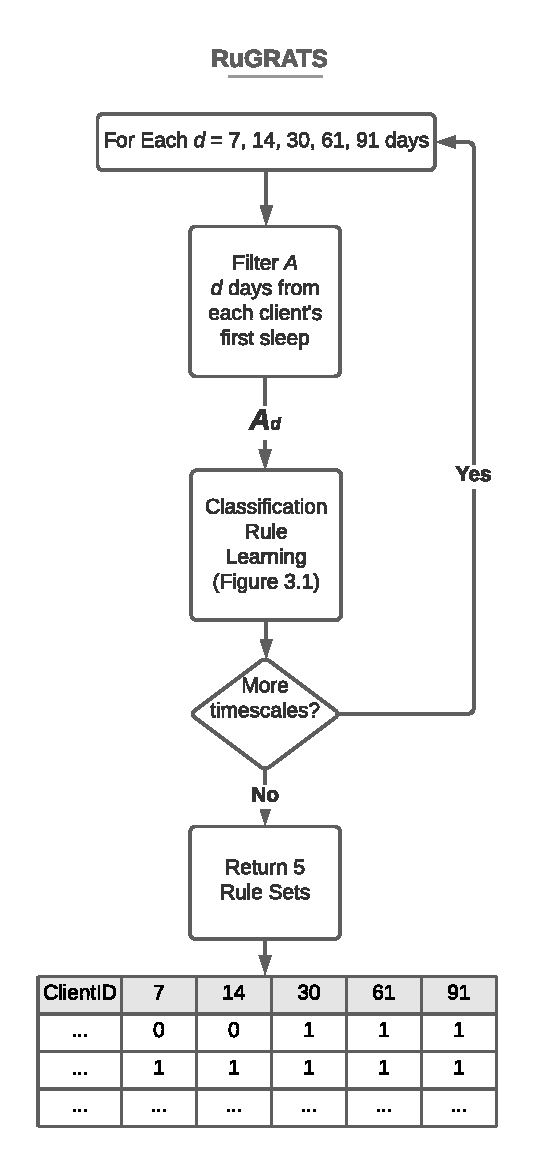
\includegraphics[width=0.5\textwidth]{Figures/RuGRATS.pdf}
    \caption{A high-level overview of the proposed algorithm structure.}
		\label{fig:highlevel}
\end{figure}

The outer stage (Figure \ref{fig:highlevel}) is proposed in this work as a means to identify potentially chronic individuals as early as possible. The general function of this loop is to extend the concept of rule sets, to \emph{time-dependent} rule sets. Which when combined allow the \Abb recommendation system to identify clients very rapidly at short time scales, while still taking advantage of the availability of data after a longer period.

Time-dependent rule sets are rule sets that are only exposed to a client's first $d$ days sleeping in shelter. Thus, the outer loop in Figure \ref{fig:highlevel} loops over a set number of time scales. In this work $d =$ 7, 14, 30, 61, and 91 days. This outer loop will generate five time-dependent rule sets, one for each value of $d$. The \Abb system will return a matrix of classifications (see Figure \ref{fig:highlevel}), with one client per row, and the columns represent after how many days the client was identified to be potentially chronic. In the figure, 0 refers to not identified, and 1 is identified. The proposed system would re-generate the matrix of classifications every day using updated data from each client. The five rule sets could also be updated daily, or updated periodically.
Section \ref{chap:algo:proposed} covers this concept in more detail and introduces a metric (Section \ref{chap:algo:mtti}) that can aid in comparing the rapidity of classification. This metric will approximate the mean identification time of a given classifier allowing multiple classifiers to be compared.

The inner stage is a typical rule set learning system (Figure \ref{fig:covering}) with a focus on simple, easy-to-understand operations. This stage employs the weighted covering algorithm (Section \ref{chap:algo:weightcov}), which repeatedly uses the Apriori algorithm to generate the top rule (Section \ref{chap:algo:whypriori}). The Apriori stage composes rules made up of features generated in the feature generation stage (Section \ref{chap:algo:binning}).
This inner stage can easily be replaced by another classification system (e.g. Logistic Regression, Neural Network etc.). Replacing the inner stage might be useful for a homeless shelter that is willing to forgo interpretability for more performant classifications. The inner stage presented here is designed to be simple with an interpretable output. As discussed in Chapter \ref{chap:intro}, classification rule learning excels in interpretability because all decision making in the classifier is encoded into a rule set.

\section{Feature Generation} \label{chap:algo:binning}

The feature format selected for this is the threshold method mentioned in Section \ref{chap:rule:pre}. Features will take the form $a < \theta$ and $a \geq \theta$ where $\theta$ is a value in the range $[1, max(a)]$ for each attribute $a$. This form was chosen carefully to avoid over-fitting and increase the fairness of classification. Features of the form $a = \theta$ will have less coverage than a rule of the form $a \geq \theta$ because they are more specific, thus leading to over-fitting. The fairness of open-ended features comes naturally from the fact that they are open-ended. For example, the feature $Sleep = 29$ will only represent clients with exactly 29 sleeps. A client with more than 29 nights in shelter would not be identified by this rule when in reality they have more nights in shelter.


The feature generation process was designed to limit the number of features generated per attribute to ten or less. As was discussed in Chapter \ref{chap:rule}, having a large number of features exponentially increases the search space of rule learning, and the time it takes to generate rule sets. The cutoff of ten features was put in place to minimize generation time, and still provide some granularity of features.
The values of $\theta$ are based on the range of attribute $a$, if $max(a) \leq 20$ then $\theta = 2n + 1 \text{ where } n \in [1, \frac{max(a)}{2} + 1]$. If $max(a) > 20$ then $\theta$ is an exponentially distributed variable with a value $\theta = \lfloor e^\frac{n\log(max(a))}{10} \rfloor \text{ where } n \in  [0, 10]$. This distribution was chosen to match the typical distribution of attributes in $A$ (shown in Figure \ref{fig:pdf}) and give features a higher resolution in the lower ranges, which represent a larger proportion of clients.
The feature reduction techniques presented in Section \ref{chap:rule:pre} are not used in this work because the above technique sufficiently reduces the number of features. The second technique presented in Section \ref{chap:rule:pre} is not needed because it is made redundant by the use of the Apriori algorithm (Section \ref{chap:algo:whypriori}).


% Table \ref{tbl:algo:examplefeatures} demonstrates some actual features used by the \Abb system. These are randomly selected features, and are specifically generated with $d=30$. For convenience, features of the form $a < 1$ are represented as 'No $a$'.

% \begin{table}[h]
% 	\centering

% 	\begin{tabular}{c}
% 	\toprule
% 	EmployeeIsCounsellor $< 3$ \\
% 	Sleep $\geq 23$ \\
% 	Age $\geq 50$ \\
% 	No Log \\

% 	\bottomrule
% 	\end{tabular}

% 	\caption{Example features.}
% 	\label{tbl:algo:examplefeatures}
% \end{table}


\section{Top Rule Learning}\label{chap:algo:whypriori}

In this work, the Apriori algorithm will be used to search for possible rules. As discussed in Chapter \ref{chap:rule}, the Apriori algorithm is very similar to the BFS exhaustive search but has the additional heuristic that it drops rules with low coverage. Dropping rules with low coverage during the search procedure reduces the search space and allows the Apriori algorithm to discover rules more efficiently. As rule length increases, rule coverage goes down (discussed in Section \ref{chap:rule:pre}), this means that dropping low coverage rules early on in the search procedure will not preclude further high-quality rules from being generated. 

The reason for using a heuristic based on exhaustive search is to combat the myopia present in hill search and beam search techniques. These algorithms do not search the entire space of possible rules and thus can get stuck in local maxima and will be unable to find the best rule. The typical reason to implement hill climbing or beam search is to discover rules with a larger depth.

Rules with a larger depth are "specific", this is in contrast to shorter rules which are "general". The terms specific and general refer to the implied coverage of a rule. That is, a rule with a large depth will have many features, with each added feature reducing the coverage, meaning that longer rules will typically have lower coverage than a similar short rule. Short rules cover general populations, for example, Sleep $>30$ is more general than Sleep $> 30$ AND Log $< 15$ because it describes a more generic population. Rules with a larger depth are therefore at risk of over-fitting. In this work, a rule depth limit of 2 is employed. This limit is in place to prevent over-fitting (and focus on more general rules), but the exact value was chosen based on computing constraints (going to a depth of 3 required 50x the computing time). An implemented system would not have the computing time constraint and could use a slightly larger depth.

% 20:35:52.269123
% vs.
% 0:24:21.123328

% 2. Exhaustive search techniques are easy to explain to the layperson user of the system. Other search heuristics, such as hill climbing and beam search require specific knowledge about searching to understand. By contrast, an explanation of the Apriori algorithm can be truthfully simplified as "All possible rules are generated, and the top rule that covers at least N clients is selected". This hides some implementation details of the Apriori algorithm, but still reflects what is happening and the intuition that a user develops will be true. Hill climbing and beam search can not be simplified in such a way, and if the above explanation is used, these techniques could return rules that do not intuitively make sense to a shelter operator (in the worst case of both algorithms, the local maxima is followed until a non-optimal solution is found).



Traditionally the Apriori algorithm uses the Precision measure to rank rules. For this work, other measures were considered with the goal of improving classification performance. Appendix \ref{chap:perf} compares six different performance measures in the context of this work. Ultimately, the Apriori measures, Support, Precision (Confidence), and Lift were not replaced because of their tolerance to data sets with class imbalance and the intuitive nature of the rules (e.g. for Lift any value above 1 is better than a random guess).

% \tdo{How can I integrate this table?}
% Table \ref{tbl:algo:examplerules} demonstrates an example rule set made up of rules that have been generated using this procedure. Again, these rules were generated with $d=30$.

% \begin{table}[h]
% 	\centering

% 	\begin{tabular}{c}
% 	\toprule
% 	Age $\geq 50$ AND Sleep $\geq 29$ \\
% 	No Log AND Sleep $\geq 29$ \\
% 	Age $\geq 50$ AND Sleep $\geq 25$ \\
% 	Age $\geq 42$ AND Sleep $\geq 27$ \\
% 	EmployeeIsCounsellor $< 3$ AND Sleep $\geq 27$ \\
% 	Age $\geq 42$ AND Sleep $\geq 21$ \\

% 	\bottomrule
% 	\end{tabular}

% 	\caption{Example rule set.}
% 	\label{tbl:algo:examplerules}
% \end{table}

\section{Rule Set Learning}\label{chap:algo:weightcov}

The standard for rule learning is to use some variant of the covering algorithm. This work is no different and employs the weighted covering algorithm to generate rule sets. This choice was made to increase the redundancy of the generated rule sets.
The redundancy of the weighted covering algorithm allows a client to be covered $k$ times before being removed from consideration. This redundancy can help reduce the problem of over-fitting. In this work $k$ was chosen to be 5, this variable is available to be optimized but was not in this work. Following the recommendation in \cite{lavrac2004weighted}, the additive weighting scheme was used. A factor in the decision for using this scheme is the simplicity and the goal of maintaining simplicity wherever possible.

The use of the weighted covering algorithm necessitates that the implementation of Support, Precision, and Lift must take the weight of each client into account. Let $P(R)$ be the probability that a given rule classifies a client as chronic, $P(C)$ is the probability that a client actually is chronic, and $P(R \cap C)$ is the probability that a client is chronic and identified as such. $P(R) = \frac{n(R)}{N}$, $P(C) = \frac{n(c)}{N}$, and $P(R \cap C) = \frac{n(R \cdot C)}{N}$ where $n(R)$ is the number of clients identified by a given rule, $n(C)$ is the number of chronic clients, $n(R \cdot C)$ is the number of clients that are chronic and identified as such, and $N$ is the total number of clients, this follows the convention in \cite{lavrac2004weighted}. The definitions of Support, Precision, and Lift are $P(R \cap C) = \frac{n(R \cdot C)}{N}$, $P(C|R) = \frac{n(R \cdot C)}{n(R)}$, and $\frac{P(C|R)}{P(C)} = \frac{n(R \cdot C) \cdot N}{n(R) \cdot n(C)}$ respectively. In order to take weight into account, $n(R)$, $n(C)$, $n(R \cdot C)$, and $N$ will be substituted with $n'(R)$, $n'(C)$, $n'(R \cdot C)$, and $N'$. Where $N'$ is the summation of all clients weights and $n'(R)$, $n'(C)$, and $n'(R \cdot C)$ are the summation of weights of clients identified by a rule, chronic clients, and both respectively. The new definitions for Support, Precision, and Lift are $P(R \cap C) \to \frac{n'(R \cdot C)}{N'}$, $P(C|R) \to \frac{n'(R \cdot C)}{n'(R)}$, and $\frac{P(C|R)}{P(C)} \to \frac{n'(R \cdot C) \cdot N'}{n'(R) \cdot n'(C)}$ respectively.


Section \ref{chap:rule:sets} introduced the most basic stopping condition, 100\% coverage. In the \Abb system one more stopping condition is used, the minimum lift condition. A rule with a Lift of 1 has the same Precision as a random guess. Thus, if the top rule has a Lift of 1 or less, the covering algorithm can safely quit (there are no more good rules). In this work, the minimum lift is configurable and will be used by the outer loop to adjust the Precision of the resulting rule set. Precision measures the probability that a client becomes chronic given that they were classified as such. The Precision of a random guess in this data set is 4.82\% (the proportion of chronic clients) and any rule set Precision higher than that can be considered "good". Lift measures the improvement of Precision over a random guess, in this work, Lift is defined as $\frac{\text{Precision}}{4.82\%}$. A higher minimum lift will increase the overall Precision of a rule set by limiting rules with low Precision/Lift.
However, a user of the system may want much more than 4.82\% Precision in decision making. Moreover, as Precision increases, coverage tends to decrease. That is, increasing the Minimum Lift Threshold will reduce the number of clients identified as chronic, but the correct proportion of identified clients will be higher. This is useful for shelter operators, as it will allow them to increase and decrease the number of identified clients based on the available resources at the time.

The rule sets presented in Table \ref{tbl:algo:exampleminlift} were generated using this procedure. Specifically, they were generated using a Minimum Lift Threshold of 2.5 and 10.6. One thing that is evident by observing this example rule set is that the Sleep attribute seems to be the most important attribute making a chronic classification. This is understandable, as the definition used to generate the chronic labels (the DI definition, Section \ref{chap:data:labelling}) is purely based on the amount of sleep. Beyond that, it is worth noting that features based on the same attribute (e.g. Sleep $\geq 25$ and Sleep $\geq 27$) are not allowed in the same rule, but are allowed in the same rule set.

As the Minimum Lift Threshold is an early stopping condition it will affect the number of rules in a generated rule set. Table \ref{tbl:algo:exampleminlift} demonstrates this with two rule sets with a Minimum Lift Threshold of 2.5 and 10.6. As can be seen, the higher Minimum Lift Threshold significantly reduces the length of the generated rule set. These rule sets are selected examples that were generated as part of the results in Chapter \ref{chap:results}.

\begin{table}[h]
	\centering

	\begin{tabular}{cc}
	\toprule
	2.5 & 10.6 \\
	\midrule
	Age $\geq 59$ AND Sleep $\geq 27$ & Age $\geq 59$ AND Sleep $\geq 27$ \\
	Age $\geq 50$ AND Sleep $\geq 29$ & \\
	No Log AND Sleep $\geq 29$ & \\
	Age $\geq 42$ AND Sleep $\geq 25$ & \\
	EmployeeIsCounsellor $< 3$ AND Sleep $\geq 27$ & \\
	Age $\geq 50$ AND Sleep $\geq 21$ & \\
	\bottomrule
	\end{tabular}

	\caption{Example rule sets generated with Minimum Lift Thresholds of 2.5 and 10.6.}
	\label{tbl:algo:exampleminlift}
\end{table}


\section{Outer Covering Loop} \label{chap:algo:proposed}


The \Abb system proposes an outer covering loop to minimize the amount of time before a chronic classification can take place. To do this, multiple rule sets are generated where each rule set is generated using a modified attribute table with a different number of days $d$. This work uses $d$ values of 7, 14, 30, 61, and 91. These values can likely be optimized, but in the interest of simplicity, these are suitable for experimental demonstration. If this system were to be deployed, alternative values would be investigated. 

The generation process of \Abb is simply repeated generation of rule sets with the different values of $d$. If a single rule set were used the user or system designer would be presented with a trade-off. A small value of $d$ results in more rapid classification time, but lower coverage and potentially lower Precision. A large value of $d$ has better coverage and potentially better Precision, but suffers from the longer classification time. This work removes that trade-off by generating multiple rule sets. 


However, removing this trade-off does not come free. The system designer (or user) is now responsible for determining the minimum lift condition for each of the five rule sets generated in the \Abb system (as opposed to just one). In this work, three methods for determining these values are proposed. The first is the Lazy approach, this approach has the user set a minimum lift value for all rule sets. The second is the Greedy approach which selects minimum lift values that maximize the Precision for each rule set. These values are chosen by sweeping the Minimum Lift Threshold and selecting the value that maximizes the rule set Precision.
The rule sets generated by the Lazy system will tend to be longer than those generated by the Greedy system because the Minimum Lift Threshold will tend to be lower.
Thus the Greedy system will identify fewer clients than the Lazy system, but the identified clients have a higher probability of being chronic. The third approach is to leave setting the Minimum Lift Threshold values up to the user. This approach is, of course, difficult to evaluate in advance but allows a user to best tailor the system to the current needs of a shelter and its clients. Chapter \ref{chap:results} will evaluate the Lazy and Greedy methods.


Using the \Abb system to generate predictions is much the same as using a single rule set. The difference is that the order of evaluations will need to be considered. That is, in this work, five different time scales are used, meaning five different lists of clients will be identified as at risk to become chronic. The user of the system will need to manually determine the prioritization of clients across these lists. This is considered a benefit as it allows the system to mesh with shelter operations and allows a human to have the final say on critical decisions such as housing. This is particularly important for shelter operators because it will allow them to limit the number of False Positives when housing resources are scarce and it allows them to identify more clients when housing resources are available.

An effect of generating rule sets using different time scales is that the generated rule sets will have a different number of rules and likely a different diversity of rules. Table \ref{tbl:algo:exampledays} demonstrates this with two rule sets, one generated with $d=7$ and the other with $d=91$. As can be expected the rules in the rule set with $d=91$ are much richer, this is because there is more client data available after 91 days. A note, some rules are redundant, particularly in the $d=7$ rule set, and could be automatically removed to make the rule set more clear. This is not shown here but should be employed if this system is used. A typical cleaning method is the pruning operation discussed in Chapter \ref{chap:rule}. Another option is to simply numerically compare the overlap of the rules. For example, the $d=7$ rule set in Table \ref{tbl:algo:exampledays} can be reduced by observing that the features are the same in all rules and can be combined by taking the minimum value of each feature. Thus, the $d=7$ rule set can be reduced to the single rule Age $\geq 42$ AND Sleep $\geq 5$.

\begin{table}[h]
	\centering

	\begin{tabular}{cc}
	\toprule
	$d=7$ & $d=91$ \\
	\midrule
	Age $\geq 59$ AND Sleep $\geq 7$ & Age $\geq 42$ AND Sleep $\geq 91$ \\
	Age $\geq 50$ AND Sleep $\geq 7$ & Age $\geq 59$ AND Sleep $\geq 55$ \\
	Age $\geq 42$ AND Sleep $\geq 7$ & No EmployeeIsCounsellor AND Sleep $\geq 55$ \\
	Age $\geq 50$ AND Sleep $\geq 5$ & Age $\geq 50$ AND Sleep $\geq 55$ \\
																	 & Age $\geq 42$ AND Sleep $\geq 55$ \\
																	 & Log $< 4$ AND Sleep $\geq 55$ \\
																	 & Age $\geq 50$ AND Sleep $\geq 33$ \\

	\bottomrule
	\end{tabular}

	\caption{Example rule sets generated with different time scales, $d=7$ and $d=91$.}
	\label{tbl:algo:exampledays}
\end{table}

\subsection{Mean Time to Identification} \label{chap:algo:mtti}

The purpose of the \Abb system is to identify potentially chronic individuals as rapidly as possible. Ideally, there would be a method to measure and compare the timeliness of classification. In this work the Mean Time To Identification (MTTI) measure is proposed to do exactly this. MTTI is calculated using a loop similar to the covering algorithm, that is, the rule sets are applied to the data set one at a time starting with the smallest value of $d$. For each rule set, the number of covered chronic clients is recorded and those clients are removed from the data set. This procedure is repeated until all the rule sets have been used.
The mean of each classification time ($d$) is then taken, chronic clients who are not identified by one of the five rule sets are assumed to be classified using the DI definition (Section \ref{chap:data:labelling}). A result of using mean identification time, rather than median is that the mean identification time will be able to represent clients who are identified by the classifier and those that are not (true positives and false negatives). Having a small MTTI value is thus reflective of a classifier being able to identify a large number of individuals, and being able to identify them in shorter time scales. Chapter \ref{chap:results} will make use of this measure to compare \Abb strategies.

% Geoff commented on my second assumption asking if it was necessary.
% I feel it's necessary because in the case of some episodic clients, they are 
% "Successfully housed" but still experience episodes of homelessness afterwards
The MTTI measure does not measure the time that a client will be homeless, and does not provide any sort of guarantee as to the identification time for a specific client.
This is because MTTI makes three key assumptions. The first assumption is that clients that are identified and immediately housed after $d$ days for each rule set (e.g. the assumption is that all clients identified in the $d=7$ rule set are identified after 7 days). This assumption is false because it assumes that every client is immediately housed and does not allow for delays.
The second assumption is that clients who are identified by the system never re-enter homelessness. The assumption is not true because clients often experience multiple episodes of homelessness.
The third assumption is that clients who are not identified by the classification system will be identified after 666 days (the mean time to identification for the DI definition, Section \ref{chap:data:labelling}). This assumption is false because it only uses the mean identification time for the DI definition and does not take the distribution of identification time into account. For example, Table \ref{tbl:stats:chronic} demonstrates that the minimum time to chronic identification is 276 days, and Section \ref{chap:data:labelling} shows that the median is 349 days.
So the MTTI measure is not a completely accurate measure of identification speed. Instead, the MTTI measure provides a simple metric to compare different classification systems based on the \Abb system.


\section{Summary}

This chapter introduced the details of the \Name (\Abb) system. The feature generation, top rule learning, and rule set learning procedures were more concretely discussed and solidified. Across all stages of this system, simplicity was preferred to allow users to understand the procedures. This also extends to the outer loop of the \Abb system that functions primarily to give users insight into clients who are at risk of becoming chronic. The following chapter (Chapter \ref{chap:results}) will evaluate the \Abb system along with the \Abb rule set learning algorithm and compare it against more commonly used classification systems.

